\chapter{Testing and Analysis}
\section{System Testing}
In this chapter, will be explain about testing and analysis that used in this final project. The result of this testing and analyzing process will show how good the perfomance of the system is. There are two aspects that will be the concern in this step, they are execution time and the correctness of the outputs.  

\subsection{Testing Objective}
Based on the system model in chapter 3, the shortest path algorithms will be implemented in Indoor Routing System using three dimensional data structure. And the objectives of this testing process are:
\begin{enumerate}
%	\item Knowing that the shortest path algorithms can be implemented in three dimensional graph data structure.
	\item To get the best system's performance by comparing the execution time between Dijkstra's, Bellman-Ford, Floyd-Warshall, and A* algorithms.
	\item To get the system's accuracy by comparing the distance as the result of TELUR IRIS system and  the distance in real life.
\end{enumerate}

\subsection{Testing Scenario}
The following statements are the scenario of testing process:

\begin{enumerate}
	\item \textbf{Testing of system's perfomance in execution time}. In this section, each of dijkstra's, bellman-ford, floyd-warshall, and A* will be tested five times to get the execution time. After that the average amount can be assumed as the exact execution time. this testing will be implemented in both open and close space wich is has different count of nodes and edges.
	
	\item \textbf{Testing of system's accuracy}. In this section, comparison between the distance as the result of TELUR IRIS system and  the distance in real life will be calculated. For each scenario, there will be three samples of calculation result.
	
	The scenario of this test will be devided into 4, those are:
	\begin{itemize}
		\item Distance calculation between two rooms that have same Building\textunderscore{ID} and same $z$ attribute.
		\item Distance calculation between two rooms that have same Building\textunderscore{ID} but different $z$ attribute.
		\item Distance calculation between two rooms that have different Building\textunderscore{ID} but same $z$ attribute.
		\item Distance calculation between two rooms that have different Building\textunderscore{ID} and different $z$ attribute.
	\end{itemize}
	
\end{enumerate}

\section{Testing Result}

\subsection{Time Execution Comparison}
Here are the result of time execution testing. For the testing sample, the shortest path between node IF1.01.01 to node IF3.03.07 were choosen as a sample. This test implemented Dijkstra, Floyd-Warshall, Bellman-Ford, and A* Algorithms to search that shortest path. The testing do the searching process five times for each algorithms and it took the average value of the execution times as the result. All the time values are in seconds. 
\\\\
\textbf{The output of five times Dijkstra's Algorithm running:}\\
*****dijkstra algorithm node IF1.01.01 to IF3.03.07*****\\
graph.getNodeCount() = 272\\
execution time dijkstra : 0.176570559\\
*****dijkstra algorithm node IF1.01.01 to IF3.03.07*****\\
graph.getNodeCount() = 266\\
execution time dijkstra\textunderscore{close} : 0.059495901\\
executed in 0.23606646 seconds\\
\\
*****dijkstra algorithm node IF1.01.01 to IF3.03.07*****\\
graph.getNodeCount() = 272\\
execution time dijkstra : 0.059805929\\
*****dijkstra algorithm node IF1.01.01 to IF3.03.07*****\\
graph.getNodeCount() = 266\\
execution time dijkstra\textunderscore{close} : 0.030269795\\
executed in 0.090075724 seconds\\
\\
*****dijkstra algorithm node IF1.01.01 to IF3.03.07*****\\
graph.getNodeCount() = 272\\
execution time dijkstra : 0.048037625\\
*****dijkstra algorithm node IF1.01.01 to IF3.03.07*****\\
graph.getNodeCount() = 266\\
execution time dijkstra\textunderscore{close} : 0.035783754\\
executed in 0.083821379 seconds\\
\\
*****dijkstra algorithm node IF1.01.01 to IF3.03.07*****\\
graph.getNodeCount() = 272\\
execution time dijkstra : 0.04465599\\
*****dijkstra algorithm node IF1.01.01 to IF3.03.07*****\\
graph.getNodeCount() = 266\\
execution time dijkstra\textunderscore{close} : 0.030038336\\
executed in 0.074694326 seconds\\
\\
*****dijkstra algorithm node IF1.01.01 to IF3.03.07*****\\
graph.getNodeCount() = 272\\
execution time dijkstra : 0.06649877\\
*****dijkstra algorithm node IF1.01.01 to IF3.03.07*****\\
graph.getNodeCount() = 266\\
execution time dijkstra\textunderscore{close} : 0.032153671\\
executed in 0.098652441 seconds\\
\\\\
\textbf{The output of five times Floyd-Warshall Algorithm running:}\\
*****Floyd-Warshal algorithm node IF1.01.01 to IF3.03.07*****\\
graph.getNodeCount() = 272\\
execution time fw : 0.280716078\\
*****Floyd-Warshal algorithm node IF1.01.01 to IF3.03.07*****\\
graph.getNodeCount() = 266\\
execution time fw\textunderscore{close} : 0.175645076\\
executed in 0.456361154 seconds\\
\\
*****Floyd-Warshal algorithm node IF1.01.01 to IF3.03.07*****\\
graph.getNodeCount() = 272\\
execution time fw : 0.262804205\\
*****Floyd-Warshal algorithm node IF1.01.01 to IF3.03.07*****\\
graph.getNodeCount() = 266\\
execution time fw\textunderscore{close} : 0.100703012\\
executed in 0.363507217 seconds\\
\\
*****Floyd-Warshal algorithm node IF1.01.01 to IF3.03.07*****\\
graph.getNodeCount() = 272\\
execution time fw : 0.295337272\\
*****Floyd-Warshal algorithm node IF1.01.01 to IF3.03.07*****\\
graph.getNodeCount() = 266\\
execution time fw\textunderscore{close} : 0.081183668\\
executed in 0.37652094 seconds\\
\\
*****Floyd-Warshal algorithm node IF1.01.01 to IF3.03.07*****\\
graph.getNodeCount() = 272\\
execution time fw : 0.283726813\\
*****Floyd-Warshal algorithm node IF1.01.01 to IF3.03.07*****\\
graph.getNodeCount() = 266\\
execution time fw\textunderscore{close} : 0.238191704\\
executed in 0.521918517 seconds\\
\\
*****Floyd-Warshal algorithm node IF1.01.01 to IF3.03.07*****\\
graph.getNodeCount() = 272\\
execution time fw : 0.282648442\\
*****Floyd-Warshal algorithm node IF1.01.01 to IF3.03.07*****\\
graph.getNodeCount() = 266\\
\\execution time fw\textunderscore{close} : 0.263365865
\\executed in 0.546014307 seconds
\\\\
\\\textbf{The output of five times Bellman-Ford Algorithm running:}
\\*****Bellman-Ford algorithm node IF1.01.01 to IF3.03.07*****
\\graph.getNodeCount() = 272
\\execution time bf : 0.337928182
\\*****Bellman-Ford algorithm node IF1.01.01 to IF3.03.07*****
\\graph.getNodeCount() = 266
\\execution time bf\textunderscore{close} : 0.188902291
\\executed in 0.526830473 seconds
\\
\\*****Bellman-Ford algorithm node IF1.01.01 to IF3.03.07*****
\\graph.getNodeCount() = 272
\\execution time bf : 0.221083213
\\*****Bellman-Ford algorithm node IF1.01.01 to IF3.03.07*****
\\graph.getNodeCount() = 266
\\execution time bf\textunderscore{close} : 0.234484116
\\executed in 0.455567329 seconds
\\
\\*****Bellman-Ford algorithm node IF1.01.01 to IF3.03.07*****
\\graph.getNodeCount() = 272
\\execution time bf : 0.29284962
\\*****Bellman-Ford algorithm node IF1.01.01 to IF3.03.07*****
\\graph.getNodeCount() = 266
\\execution time bf\textunderscore{close} : 0.240597956
\\executed in 0.533447576 seconds
\\
\\*****Bellman-Ford algorithm node IF1.01.01 to IF3.03.07*****
\\graph.getNodeCount() = 272
\\execution time bf : 0.273845218
\\*****Bellman-Ford algorithm node IF1.01.01 to IF3.03.07*****
\\graph.getNodeCount() = 266
\\execution time bf\textunderscore{close} : 0.246817972
\\executed in 0.52066319 seconds
\\
\\*****Bellman-Ford algorithm node IF1.01.01 to IF3.03.07*****
\\graph.getNodeCount() = 272
\\execution time bf : 0.28561423
\\*****Bellman-Ford algorithm node IF1.01.01 to IF3.03.07*****
\\graph.getNodeCount() = 266
\\execution time bf\textunderscore{close} : 0.236419664
\\executed in 0.522033894 seconds
\\\\
\\\textbf{The output of five times A* Algorithm running:}
\\*****A* algorithm node IF1.01.01 to IF3.03.07*****
\\graph.getNodeCount() = 272
\\execution time astar : 0.065852526
\\*****A* algorithm node IF1.01.01 to IF3.03.07*****
\\graph.getNodeCount() = 266
\\execution time astar\textunderscore{close} : 0.016076835
\\executed in 0.081929361 seconds
\\
\\*****A* algorithm node IF1.01.01 to IF3.03.07*****
\\graph.getNodeCount() = 272
\\execution time astar : 0.03272878
\\*****A* algorithm node IF1.01.01 to IF3.03.07*****
\\graph.getNodeCount() = 266
\\execution time astar\textunderscore{close} : 0.023422293
\\executed in 0.056151073 seconds
\\
\\*****A* algorithm node IF1.01.01 to IF3.03.07*****
\\graph.getNodeCount() = 272
\\execution time astar : 0.030558941
\\*****A* algorithm node IF1.01.01 to IF3.03.07*****
\\graph.getNodeCount() = 266
\\execution time astar\textunderscore{close} : 0.01713822
\\executed in 0.047697161 seconds
\\
\\*****A* algorithm node IF1.01.01 to IF3.03.07*****
\\graph.getNodeCount() = 272
\\execution time astar : 0.026007271
\\*****A* algorithm node IF1.01.01 to IF3.03.07*****
\\graph.getNodeCount() = 266
\\execution time astar\textunderscore{close} : 0.022123787
\\executed in 0.048131058 seconds
\\
\\*****A* algorithm node IF1.01.01 to IF3.03.07*****
\\graph.getNodeCount() = 272
\\execution time astar : 0.036428937
\\*****A* algorithm node IF1.01.01 to IF3.03.07*****
\\graph.getNodeCount() = 266
\\execution time astar\textunderscore{close} : 0.032021663
\\executed in 0.0684506 seconds
\\\\

The tables below shows the clearer comparison according to the console output of the system above. Table \ref{table:2} shows the comparison of the shortest path algorithms in showing the actual shortest path where all nodes (total 272 nodes) of the graph are included in the algorithm's calculation. Table \ref{table:3} shows the comparison of the shortest path algorithms in showing the shortest path in close space where nodes wich are the open space will not be calculated in shortest path algorithm (total 266 nodes).


% Please add the following required packages to your document preamble:
% \usepackage[table,xcdraw]{xcolor}
% If you use beamer only pass "xcolor=table" option, i.e. \documentclass[xcolor=table]{beamer}
\begin{table}[h!]
	\centering
	\caption{Shortest path execution time comparison for Whole Space}
	\label{table:2}
	\begin{tabular}{|c|l|l|l|l|}
		\hline
		\textbf{Itteration}                                            & \multicolumn{1}{c|}{\textbf{Dijkstra}} & \multicolumn{1}{c|}{\textbf{Floyd-Warshall}} & \multicolumn{1}{c|}{\textbf{Bellman-Ford}} & \multicolumn{1}{c|}{\textbf{A*}} \\ \hline
		1                                                              & 0.176570559                            & 0.280716078                                  & 0.337928182                                & 0.065852526                      \\ \hline
		2                                                              & 0.059805929                            & 0.262804205                                  & 0.221083213                                & 0.03272878                       \\ \hline
		3                                                              & 0.048037625                            & 0.295337272                                  & 0.29284962                                 & 0.030558941                      \\ \hline
		4                                                              & 0.04465599                             & 0.283726813                                  & 0.273845218                                & 0.026007271                      \\ \hline
		5                                                              & 0.06649877                             & 0.282648442                                  & 0.28561423                                 & 0.036428937                      \\ \hline
		\rowcolor[HTML]{9B9B9B} 
		\multicolumn{1}{|l|}{\cellcolor[HTML]{9B9B9B}\textbf{AVERAGE}} & 0.079113775                            & 0.281046562                                  & 0.282264093                                & 0.038315291                      \\ \hline
	\end{tabular}
\end{table}

% Please add the following required packages to your document preamble:
% \usepackage[table,xcdraw]{xcolor}
% If you use beamer only pass "xcolor=table" option, i.e. \documentclass[xcolor=table]{beamer}
\begin{table}[h!]
	\centering
	\caption{Shortest path execution time comparison for Close Space}
	\label{table:3}
	\begin{tabular}{|c|l|l|l|l|}
		\hline
		\textbf{Itteration}                                            & \multicolumn{1}{c|}{\textbf{Dijkstra}} & \multicolumn{1}{c|}{\textbf{Floyd-Warshall}} & \multicolumn{1}{c|}{\textbf{Bellman-Ford}} & \multicolumn{1}{c|}{\textbf{A*}} \\ \hline
		1                                                              & 0.059495901                            & 0.175645076                                  & 0.188902291                                & 0.016076835                      \\ \hline
		2                                                              & 0.030269795                            & 0.100703012                                  & 0.234484116                                & 0.023422293                      \\ \hline
		3                                                              & 0.035783754                            & 0.081183668                                  & 0.240597956                                & 0.01713822                       \\ \hline
		4                                                              & 0.030038336                            & 0.238191704                                  & 0.246817972                                & 0.022123787                      \\ \hline
		5                                                              & 0.032153671                            & 0.263365865                                  & 0.236419664                                & 0.032021663                      \\ \hline
		\rowcolor[HTML]{9B9B9B} 
		\multicolumn{1}{|l|}{\cellcolor[HTML]{9B9B9B}\textbf{AVERAGE}} & 0.037548291                            & 0.171817865                                  & 0.2294444                                  & 0.02215656                       \\ \hline
	\end{tabular}
\end{table}
\vspace{8mm}
And since the system will give both open and close space shortest paths, the comparison of system's time execution will be the total value of both situation. The value are shown in Table \ref{table:4}.

% Please add the following required packages to your document preamble:
% \usepackage[table,xcdraw]{xcolor}
% If you use beamer only pass "xcolor=table" option, i.e. \documentclass[xcolor=table]{beamer}
\begin{table}[h!]
	\centering
	\caption{System's execution time comparison}
	\label{table:4}
	\begin{tabular}{|c|l|l|l|l|}
		\hline
		\textbf{Itteration}                                            & \multicolumn{1}{c|}{\textbf{Dijkstra}} & \multicolumn{1}{c|}{\textbf{Floyd-Warshall}} & \multicolumn{1}{c|}{\textbf{Bellman-Ford}} & \multicolumn{1}{c|}{\textbf{A*}} \\ \hline
		1                                                              & 0.23606646                             & 0.456361154                                  & 0.526830473                                & 0.081929361                      \\ \hline
		2                                                              & 0.090075724                            & 0.363507217                                  & 0.455567329                                & 0.056151073                      \\ \hline
		3                                                              & 0.083821379                            & 0.37652094                                   & 0.533447576                                & 0.047697161                      \\ \hline
		4                                                              & 0.074694326                            & 0.521918517                                  & 0.52066319                                 & 0.048131058                      \\ \hline
		5                                                              & 0.098652441                            & 0.546014307                                  & 0.522033894                                & 0.0684506                        \\ \hline
		\rowcolor[HTML]{9B9B9B} 
		\multicolumn{1}{|l|}{\cellcolor[HTML]{9B9B9B}\textbf{AVERAGE}} & 0.116662066                            & 0.452864427                                  & 0.511708492                                & 0.02215656                       \\ \hline
	\end{tabular}
\end{table}

According to the data above, pictures below are the chart figures that show how far are the execution time deviation between each shortest path algorithms.

\begin{figure}[h!]
	\centering
	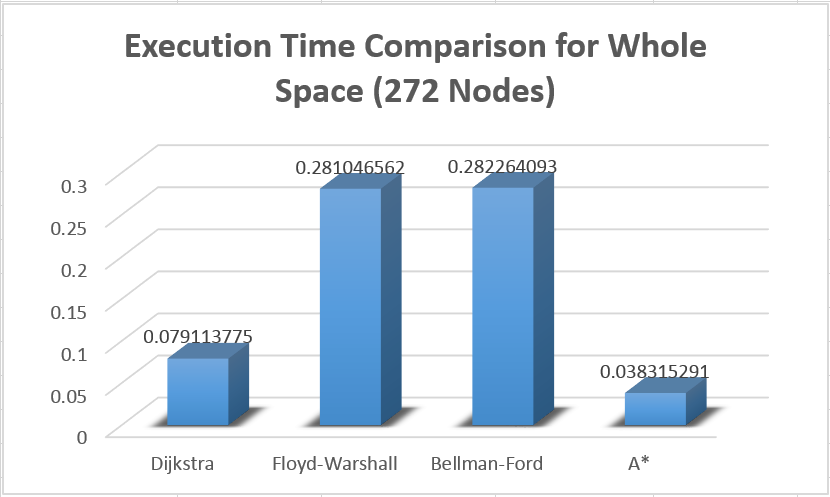
\includegraphics[scale=0.4]{graf1.PNG}
	\caption{Execution Time Comparison for Whole Space}
	\label{fig:graf1}
\end{figure}

\begin{figure}[h!]
	\centering
	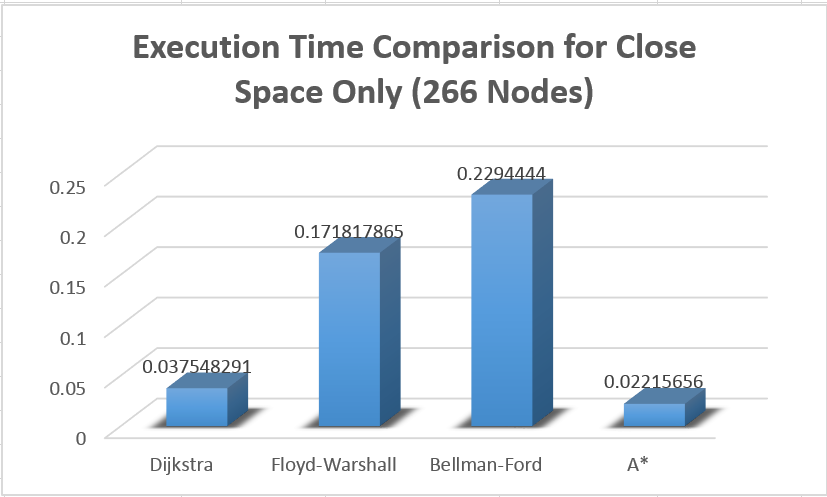
\includegraphics[scale=0.4]{graf2.PNG}
	\caption{Execution Time Comparison for Close Space Only}
	\label{fig:graf2}
\end{figure}

\begin{figure}[h!]
	\centering
	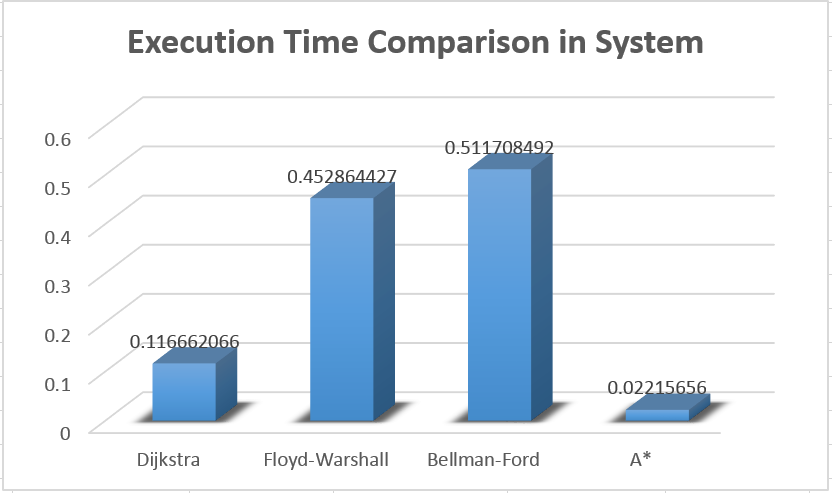
\includegraphics[scale=0.4]{graf3.PNG}
	\caption{Execution Time Comparison in System
	}
	\label{fig:graf3}
\end{figure}

\vspace{10mm}
As seen in the charts above, it could be concluded that A* Algorithm give the smallest execution time wich mean A* algorithm is the best algorithm to implement in this case besides Dijkstra, Floyd-Warshall, or Bellman-Ford algorithm. 
\vspace{60mm}
\subsection{Distance Calculation Comparison}
Here are the result of the system's accuracy testing. This testing will show the deviation between the result of system calculation and the real distance as shown in Table \ref{table:6}. All the distances are in meters.

% Please add the following required packages to your document preamble:
% \usepackage[table,xcdraw]{xcolor}
% If you use beamer only pass "xcolor=table" option, i.e. \documentclass[xcolor=table]{beamer}
\begin{table}[h!]
	\centering
	\caption{Distance deviation between system result and in the real life}
	\label{table:6}
	\begin{tabular}{|c|l|l|l|l|l|}
		\hline
		\rowcolor[HTML]{C0C0C0} 
		\textbf{No.} & \multicolumn{1}{c|}{\cellcolor[HTML]{C0C0C0}\textbf{Source}} & \multicolumn{1}{c|}{\cellcolor[HTML]{C0C0C0}\textbf{Destination}} & \multicolumn{1}{c|}{\cellcolor[HTML]{C0C0C0}\textbf{SPD\_S}} & \multicolumn{1}{c|}{\cellcolor[HTML]{C0C0C0}\textbf{SPD\_R}} & \multicolumn{1}{c|}{\cellcolor[HTML]{C0C0C0}\textbf{\begin{tabular}[c]{@{}c@{}}Deviation \\ ($ABS\left( SP\_S-SP\_R\right)$ )\end{tabular}}} \\ \hline
		1            & IF3.03.04                                                    & IF3.03.05                                                         & 8.661221996                                                  & 6                                                            & \cellcolor[HTML]{FFFC9E}2.661221996                                                                                        \\ \hline
		2            & IF3.02.05                                                    & IF3.02.01                                                         & 34.78388051                                                  & 34.7                                                         & \cellcolor[HTML]{FFFC9E}0.083880508                                                                                        \\ \hline
		3            & IF3.01.02                                                    & IF3.01.03                                                         & 21.56047226                                                  & 21.7                                                         & \cellcolor[HTML]{FFFC9E}0.139527743                                                                                        \\ \hline
		4            & IF3.03.03                                                    & IF3.02.05                                                         & 38.7783564                                                   & 34.1                                                         & \cellcolor[HTML]{FFFC9E}4.6783564                                                                                          \\ \hline
		5            & IF3.03.03                                                    & IF3.01.05                                                         & 41.18405404                                                  & 35.4                                                         & \cellcolor[HTML]{FFFC9E}5.784054043                                                                                        \\ \hline
		\rowcolor[HTML]{FFFFFF} 
		6            & IF2.01.10                                                    & IF2.02.09                                                         & 36.66114963                                                  & 31                                                           & 5.661149626                                                                                        \\ \hline
		7            & IF2.01.10                                                    & IF3.01.08                                                         & 102.1953267                                                  & 89.4                                                         & \cellcolor[HTML]{FFFC9E}12.79532672                                                                                        \\ \hline
	\end{tabular}
\end{table}

Figure \ref{fig:graf3} shows the fluctuation of the testing deviation result. From the chart, we can see that the daviation result is quiet fluctuate. This result means that this system has a deficiency in resuting the distance with average deviation velue is 4.543359576 meters.


\begin{figure}[h!]
	\centering
	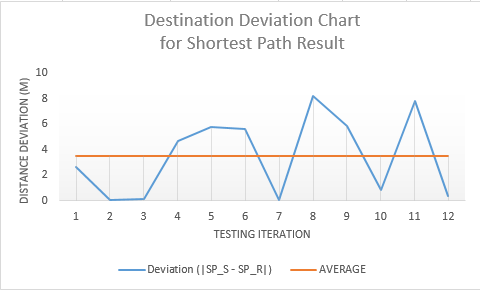
\includegraphics[scale=1]{graf4.PNG}
	\caption{Distance deviation testing result 
	}
	\label{fig:graf3}
\end{figure}

\section{Summary}
